\documentclass[12pt]{article}

\usepackage[margin=1in]{geometry}
\usepackage{amsmath,amssymb,mathtools}
\usepackage{tikz}
\usepackage{graphicx}
\usepackage{float}
\usepackage{enumitem}
\usepackage{booktabs}
\newcommand{\answer}[1]{\boxed{\;#1\;}}

\setlength{\parindent}{0pt}
\setlength{\parskip}{0.6em}

\title{EE 115 -- Homework 2}
\author{Kaushik Vada}
\date{\today}

\begin{document}

\maketitle

\section*{Problem 1}

The passband signal is
\[
  x(t) = 3\bigl(\sin(100\pi t) + \sin(200\pi t)\bigr)\cos(1000\pi t)
       = m(t)\cos(1000\pi t),
\]
where $m(t) = 3\bigl(\sin(100\pi t) + \sin(200\pi t)\bigr)$ carries baseband components at $50\,\text{Hz}$ and $100\,\text{Hz}$.  The channel $h(t)$ is an ideal lowpass filter with
\[
H(f) = \operatorname{rect}\!\left(\frac{f}{220}\right) =
  \begin{cases}
    1, & |f| < 110~\text{Hz},\\
    0, & |f| > 110~\text{Hz}.
  \end{cases}
\]
Multiplication by a sinusoid in time shifts the spectrum in frequency; the output of $h(t)$ therefore keeps only those shifted components that fall inside $|f|<110\,\text{Hz}$.

\begin{enumerate}[label=\textbf{(\alph*)}]
  \item
    \[
      y_1(t)
      = h(t) * \bigl[x(t)\cos(1000\pi t)\bigr]
      = h(t) * \bigl[m(t)\cos^2(1000\pi t)\bigr].
    \]
    Using $\cos^2\theta = \tfrac{1}{2}\left(1+\cos 2\theta\right)$, the term at $2\cdot500=1000\,\text{Hz}$ is rejected by $H(f)$, leaving
    \[
      y_1(t) = \frac{1}{2}m(t)
              = \frac{3}{2}\bigl(\sin(100\pi t) + \sin(200\pi t)\bigr).
    \]
    \emph{Work.} Using the identity
    \[
      \cos(1000\pi t)\cos(1000\pi t)=\tfrac{1}{2}\!\left(1+\cos(2000\pi t)\right),
    \]
    we write
    \[
      x(t)\cos(1000\pi t) = m(t)\cos^2(1000\pi t)
      = \tfrac{1}{2}m(t) + \tfrac{1}{2}m(t)\cos(2000\pi t).
    \]
    Multiplication by \(\cos(2000\pi t)\) shifts the baseband spectrum of \(m(t)\) to \(\pm 1000\,\text{Hz}\), which lies outside the low-pass passband \(|f|<110\,\text{Hz}\). Hence the filter removes that term and passes only \(\tfrac{1}{2}m(t)\).

    \[
      \answer{y_1(t)=\tfrac{1}{2}m(t)=\tfrac{3}{2}\bigl(\sin(100\pi t)+\sin(200\pi t)\bigr)}
    \]

  \item
    \[
      y_2(t) = h(t) * \bigl[m(t)\cos(1000\pi t)\cos(1000\pi t+\tfrac{\pi}{4})\bigr].
    \]
    With the identity $\cos\alpha\cos\beta = \tfrac{1}{2}\bigl[\cos(\alpha-\beta) + \cos(\alpha+\beta)\bigr]$,
    \[
      \cos(1000\pi t)\cos(1000\pi t+\tfrac{\pi}{4})
      = \tfrac{1}{2}\bigl[\cos(\tfrac{\pi}{4}) + \cos(2000\pi t + \tfrac{\pi}{4})\bigr].
    \]
    The component near $1000\,\text{Hz}$ is filtered out, yielding
    \[
      y_2(t) = \frac{\sqrt{2}}{4}m(t)
              = \frac{3\sqrt{2}}{4}\bigl(\sin(100\pi t) + \sin(200\pi t)\bigr).
    \]
    \emph{Work.} Apply
    \[
      \cos\alpha\cos\beta=\tfrac{1}{2}\!\left[\cos(\alpha-\beta)+\cos(\alpha+\beta)\right].
    \]
    With \(\alpha=1000\pi t\) and \(\beta=1000\pi t+\tfrac{\pi}{4}\),
    \[
      \cos(1000\pi t)\cos(1000\pi t+\tfrac{\pi}{4})
      = \tfrac{1}{2}\!\left[\cos(\tfrac{\pi}{4})+\cos(2000\pi t+\tfrac{\pi}{4})\right].
    \]
    The second term is centred at \(\pm1000\,\text{Hz}\) and is rejected by \(H(f)\); the constant factor \(\tfrac{1}{2}\cos(\tfrac{\pi}{4})=\tfrac{\sqrt{2}}{4}\) scales \(m(t)\).

    \[
      \answer{y_2(t)=\tfrac{\sqrt{2}}{4}m(t)=\tfrac{3\sqrt{2}}{4}\bigl(\sin(100\pi t)+\sin(200\pi t)\bigr)}
    \]

  \item
    \[
      y_3(t) = h(t) * \bigl[m(t)\cos(1000\pi t)\sin(1000\pi t)\bigr]
             = h(t) * \Bigl[\frac{m(t)}{2}\sin(2000\pi t)\Bigr].
    \]
    All spectral content is centred at $\pm 1000\,\text{Hz}$, hence
    \[
      y_3(t) = 0.
    \]
    \emph{Work.} First,
    \[
      \cos(1000\pi t)\sin(1000\pi t)=\tfrac{1}{2}\sin(2000\pi t).
    \]
    Therefore \(m(t)\cos(1000\pi t)\sin(1000\pi t)=\tfrac{1}{2}m(t)\sin(2000\pi t)\), whose spectrum is the spectrum of \(m(t)\) shifted to \(\pm1000\,\text{Hz}\). Since the ideal low-pass keeps only \(|f|<110\,\text{Hz}\), the entire term is removed.

    \[
      \answer{y_3(t)=0}
    \]

  \item
    The detuned local oscillator produces
    \[
      \cos(1000\pi t)\cos(1010\pi t) = \tfrac{1}{2}\bigl[\cos(10\pi t)+\cos(2010\pi t)\bigr],
    \]
    so the lowpass output retains only the term at $5\,\text{Hz}$:
    \[
      y_4(t) = \frac{1}{2} m(t)\cos(10\pi t)
              = \frac{3}{2}\bigl(\sin(100\pi t)+\sin(200\pi t)\bigr)\cos(10\pi t).
    \]
    Expanding the product highlights the new baseband tones at $45$, $55$, $95$, and $105\,\text{Hz}$:
    \[
      y_4(t) = \frac{3}{4}\Bigl[\sin(110\pi t)+\sin(90\pi t)+\sin(210\pi t)+\sin(190\pi t)\Bigr].
    \]
    \emph{Work.} The detuned LO gives
    \[
      \cos(1000\pi t)\cos(1010\pi t)=\tfrac{1}{2}\!\left[\cos(10\pi t)+\cos(2010\pi t)\right].
    \]
    The low-pass passes only the \(5\,\text{Hz}\) factor \(\tfrac{1}{2}\cos(10\pi t)\), so
    \(y_4(t)=\tfrac{1}{2}m(t)\cos(10\pi t)\).
    Using \(\sin A\cos B=\tfrac{1}{2}\left[\sin(A{+}B)+\sin(A{-}B)\right]\) with \(A\in\{100\pi t,\,200\pi t\}\) and \(B=10\pi t\) yields the four tones at \(45,55,95,105\,\text{Hz}\).

    \[
      \answer{y_4(t)=\frac{3}{4}\Bigl[\sin(110\pi t)+\sin(90\pi t)+\sin(210\pi t)+\sin(190\pi t)\Bigr]}
    \]
\end{enumerate}

% --------- Inserted: Problem 1 spectrum sketches ---------
\subsection*{Problem 1: Spectrum sketches}
\begin{figure}[H]
  \centering
  % -------- M(f) --------
  \begin{minipage}{0.48\textwidth}
    \centering
    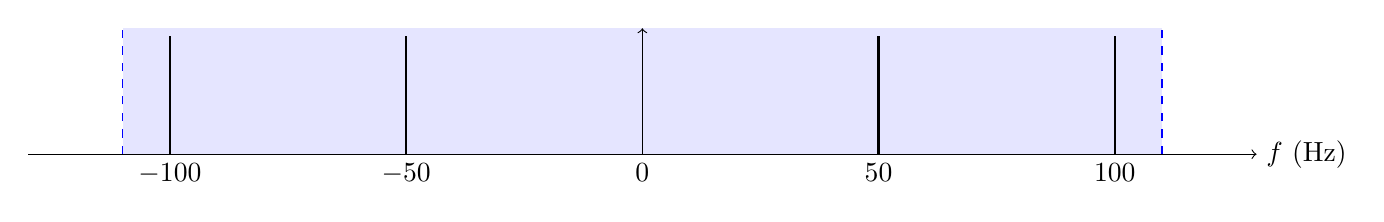
\begin{tikzpicture}[x=0.06cm,y=0.10cm]
      % axes & passband shading |f|<110
      \fill[blue!10] (-110,0) rectangle (110,16);
      \draw[dashed,blue] (-110,0)--(-110,16);
      \draw[dashed,blue] (110,0)--(110,16);
      \draw[->] (-130,0) -- (130,0) node[right] {$f$ (Hz)};
      \draw[->] (0,0) -- (0,16);
      % sticks: +/-50, +/-100 with height 1.5 -> use 15 in these units
      \foreach \f/\h in {-100/15,-50/15,50/15,100/15}{\draw[thick] (\f,0)--(\f,\h);}    
      % labels (sparse)
      \node[below] at (-100,0) {$-100$};
      \node[below] at (-50,0) {$-50$};
      \node[below] at (0,0) {$0$};
      \node[below] at (50,0) {$50$};
      \node[below] at (100,0) {$100$};
    \end{tikzpicture}\\[-0.25em]
    \small $M(f)$ (passband shaded)
  \end{minipage}\hfill
  % -------- Y1(f) --------
  \begin{minipage}{0.48\textwidth}
    \centering
    \begin{tikzpicture}[x=0.06cm,y=0.10cm]
      \draw[->] (-130,0) -- (130,0) node[right] {$f$ (Hz)};
      \draw[->] (0,0) -- (0,16);
      % height = 0.75 -> 7.5
      \foreach \f/\h in {-100/7.5,-50/7.5,50/7.5,100/7.5}{\draw[thick] (\f,0)--(\f,\h);}    
      \node[below] at (0,0) {$0$};
      \node[below] at (50,0) {$50$};
      \node[below] at (100,0) {$100$};
    \end{tikzpicture}\\[-0.25em]
    \small $Y_1(f)$
  \end{minipage}

  \vspace{0.6em}

  % -------- Y2(f) --------
  \begin{minipage}{0.48\textwidth}
    \centering
    \begin{tikzpicture}[x=0.06cm,y=0.10cm]
      \draw[->] (-130,0) -- (130,0) node[right] {$f$ (Hz)};
      \draw[->] (0,0) -- (0,16);
      % height ~ 0.5303 -> 5.3
      \foreach \f/\h in {-100/5.3,-50/5.3,50/5.3,100/5.3}{\draw[thick] (\f,0)--(\f,\h);}    
      \node[below] at (0,0) {$0$};
      \node[below] at (50,0) {$50$};
      \node[below] at (100,0) {$100$};
    \end{tikzpicture}\\[-0.25em]
    \small $Y_2(f)$
  \end{minipage}\hfill
  % -------- Y3(f) --------
  \begin{minipage}{0.48\textwidth}
    \centering
    \begin{tikzpicture}[x=0.06cm,y=0.10cm]
      \draw[->] (-130,0) -- (130,0) node[right] {$f$ (Hz)};
      \draw[->] (0,0) -- (0,16);
      % no lines (all rejected by LPF)
      \node at (0,8) {\small all suppressed};
    \end{tikzpicture}\\[-0.25em]
    \small $Y_3(f)$
  \end{minipage}

  \vspace{0.6em}

  % -------- Y4(f) --------
  \begin{minipage}{0.48\textwidth}
    \centering
    \begin{tikzpicture}[x=0.06cm,y=0.10cm]
      \draw[->] (-130,0) -- (130,0) node[right] {$f$ (Hz)};
      \draw[->] (0,0) -- (0,16);
      % lines at +/-45, +/-55, +/-95, +/-105 with height 0.375 -> 3.75
      \foreach \f in {-105,-95,-55,-45,45,55,95,105}{\draw[thick] (\f,0)--(\f,3.75);}    
      \node[below] at (-100,0) {$-100$};
      \node[below] at (-50,0) {$-50$};
      \node[below] at (0,0) {$0$};
      \node[below] at (50,0) {$50$};
      \node[below] at (100,0) {$100$};
    \end{tikzpicture}\\[-0.25em]
    \small $Y_4(f)$
  \end{minipage}

  \caption{Problem 1: stick-spectrum sketches (heights proportional to amplitude-spectrum values; $|f|<110$ Hz passband indicated on $M(f)$).}
\end{figure}

\section*{Problem 2}

The message waveform is a bipolar pulse train:
\[
  m(t) = \sum_{k=-\infty}^{\infty}\left[\operatorname{rect}(t-2k) - \operatorname{rect}(t-2k-1)\right],
\]
so $m(t)=+1$ on $(2k-\tfrac{1}{2},\,2k+\tfrac{1}{2})$ and $m(t)=-1$ on $(2k+\tfrac{1}{2},\,2k+\tfrac{3}{2})$.  The AM input to the envelope detector is $x(t) = (m(t)+\alpha)\cos(2\pi f_c t)$, and an ideal detector outputs the instantaneous envelope,
\[
  y(t) = |m(t) + \alpha|.
\]
Consequently, for any $\alpha$
\[
  y(t) =
  \begin{cases}
    |\alpha + 1|, & t \in (2k-\tfrac{1}{2},\,2k+\tfrac{1}{2}),\\
    |\alpha - 1|, & t \in (2k+\tfrac{1}{2},\,2k+\tfrac{3}{2}),
  \end{cases}
\quad k \in \mathbb{Z}.
\]
\emph{Work.} The AM input is \(x(t)=(m(t)+\alpha)\cos(2\pi f_c t)\). An ideal envelope detector outputs the instantaneous magnitude of the complex envelope, i.e., \(|m(t)+\alpha|\). Over intervals where \(m(t)=+1\) the level is \(|\alpha+1|\); where \(m(t)=-1\) the level is \(|\alpha-1|\). Special cases:
(i) \(\alpha=0\) \(\Rightarrow\) constant output \(1\) (full-wave rectification of a suppressed-carrier AM);
(ii) \(\alpha=1\) \(\Rightarrow\) the envelope just touches zero (critical modulation);
(iii) \(\alpha>1\) \(\Rightarrow\) strictly positive envelope and no sign inversions.

\[
  \answer{y(t)=|m(t)+\alpha|}
\]
\[
  \answer{\text{Levels: }|\alpha+1|\ \text{on }(2k-\tfrac{1}{2},\,2k+\tfrac{1}{2}),\quad |\alpha-1|\ \text{on }(2k+\tfrac{1}{2},\,2k+\tfrac{3}{2})}
\]

\begin{center}
  \begin{tabular}{@{}ccccc@{}}
    \toprule
    $\alpha$ & $\alpha + 1$ & $\alpha - 1$ & Output levels & Comment \\
    \midrule
    $0$   & $+1$ & $-1$  & constant $1$ & Carrier suppressed; full-wave rectification. \\
    $0.5$ & $+1.5$ & $-0.5$ & $1.5$ and $0.5$ & Unequal positive plateaus. \\
    $1$   & $+2$ & $0$    & $2$ and $0$ & Critical modulation; envelope just touches zero. \\
    $1.5$ & $+2.5$ & $+0.5$ & $2.5$ and $0.5$ & Strong carrier, always positive. \\
    \bottomrule
  \end{tabular}
\end{center}

A qualitative sketch for one period of $y(t)$ in each case is shown below (period $T=2$).

\begin{figure}[H]
  \centering
  \includegraphics[width=\textwidth]{question2_image.png}
  \caption{Envelope detector output $y(t)$ over one period ($T=2$) for $\alpha \in \{0,0.5,1,1.5\}$.}
\end{figure}

\section*{Problem 3}

The AM waveform is
\[
  x_{\text{AM}}(t) = 10\bigl(m(t) + 3\bigr)\cos(100\pi t),
\quad m(t) = \sin(20\pi t) + 2\sin(30\pi t),
\]
with carrier frequency $f_c = 50\,\text{Hz}$.

\begin{enumerate}[label=\textbf{(\alph*)}]
  \item
    \emph{Work.} Expand with product-to-sum:
    \[
    \begin{aligned}
      10(m{+}3)\cos(100\pi t)
        &= 30\cos(100\pi t) + 10\bigl[\sin(20\pi t)+2\sin(30\pi t)\bigr]\cos(100\pi t)\\
        &= 30\cos(100\pi t) \\
        &\quad + 5\!\left[\sin(120\pi t)+\sin(80\pi t)\right]
           + 10\!\left[\sin(130\pi t)+\sin(70\pi t)\right],
    \end{aligned}
    \]
    where we used \(\sin\omega_1 t\cos\omega_ct=\tfrac{1}{2}\left[\sin(\omega_c{+}\omega_1)t+\sin(\omega_c{-}\omega_1)t\right]\).
    The single-tone contributions are summarized below (Hz):
    \[
    \begin{array}{c|c|c}
      \text{Term} & \text{Frequencies} & \text{Amplitude} \\\hline
      \sin(20\pi t)\cos(100\pi t) & 50\pm 10 & 5 \\
      2\sin(30\pi t)\cos(100\pi t) & 50\pm 15 & 10 \\
      \cos(100\pi t) & 50 & 30
    \end{array}
    \]
    (For a two-sided amplitude spectrum, a cosine of amplitude \(A\) gives impulses of height \(A/2\) at \(\pm f\).)
    Expanding $x_{\text{AM}}(t)$ gives
    \[
      x_{\text{AM}}(t) = 30\cos(100\pi t)
        + 5\sin(120\pi t) - 5\sin(80\pi t)
        + 10\sin(130\pi t) - 10\sin(70\pi t).
    \]
    Therefore the (two-sided) amplitude spectrum contains impulses at the carrier and at $f_c \pm 10\,\text{Hz}$ and $f_c \pm 15\,\text{Hz}$.  Magnitudes of the spectral lines are $15$ for the carrier, $2.5$ for the $\pm 10\,\text{Hz}$ offsets, and $5$ for the $\pm 15\,\text{Hz}$ offsets:
    \[
      \begin{aligned}
        |X_{\text{AM}}(f)|
          &= 15\bigl[\delta(f-50)+\delta(f+50)\bigr] \\
          &\quad + 2.5\bigl[\delta(f-60)+\delta(f+60)+\delta(f-40)+\delta(f+40)\bigr] \\
          &\quad + 5\bigl[\delta(f-65)+\delta(f+65)+\delta(f-35)+\delta(f+35)\bigr].
      \end{aligned}
    \]
    \[
      \answer{\text{Carrier: }50~\text{Hz}@15;\ \text{Sidebands: }50\pm10~\text{Hz}@2.5,\ 50\pm15~\text{Hz}@5}
    \]
    A single-sided sketch is shown in Fig.~\ref{fig:spectrum}; the negative-frequency components mirror the positives.

    \begin{figure}[H]
      \centering
      \includegraphics[width=0.9\textwidth]{question3_image.png}
      \caption{Amplitude spectrum of $x_{AM}(t)$ showing carrier and sidebands at 50~Hz, $50\pm10$~Hz, and $50\pm15$~Hz.}
      \label{fig:spectrum}
    \end{figure}

  \item
    \emph{Work.} Write
    \[
      x_{\text{AM}}(t)=A_c\bigl[1+k_a m(t)\bigr]\cos(2\pi f_c t),\qquad
      A_c=30,\; k_a=\tfrac{1}{3},\; f_c=50~\text{Hz}.
    \]
    Since \(m(t)=\sin(20\pi t)+2\sin(30\pi t)\) attains \(\max|m(t)|=3\) and \(\min m(t)=-3\), the envelope \(A_c\bigl|1+k_a m(t)\bigr|\) just touches zero at the minimum, hence the modulation index
    \[
      \mu = k_a\,\max|m(t)| = \tfrac{1}{3}\cdot 3 = 1.
    \]
    \[
      \answer{A_c=30,\quad k_a=\tfrac{1}{3},\quad \mu=1}
    \]

  \item
    \emph{Work.} For a real sinusoid \(A\cos(\omega t)\) (or \(A\sin(\omega t)\)), the time-average power is \(A^2/2\). Orthogonality of distinct sinusoids at different frequencies makes cross-terms average to zero, so the total power is the sum of each component's \(A^2/2\). Thus the carrier contributes \(30^2/2\) and the four sidebands contribute \(5^2/2,\,5^2/2,\,10^2/2,\,10^2/2\), respectively.
    The average transmitted power equals the carrier power plus the sideband power.  From the expansion above,
    \[
      P_c = \frac{A_c^2}{2} = \frac{30^2}{2} = 450,\qquad
      P_{\text{sb}} = \frac{5^2}{2} + \frac{5^2}{2} + \frac{10^2}{2} + \frac{10^2}{2} = 125,
    \]
    giving $P_{\text{total}} = 575$.  Hence the power efficiency is
    \[
      \eta = \frac{P_{\text{sb}}}{P_{\text{total}}} = \frac{125}{575} \approx 0.217 \, (21.7\%).
    \]
    \[
      \answer{P_c=450,\quad P_{\text{sb}}=125,\quad P_{\text{total}}=575,\quad \eta=\tfrac{125}{575}\approx 0.217}
    \]
\end{enumerate}

\end{document}
